\chapter{KI}
Nedenfor følger design af software til Kontrolinterfacet. Dette er lavet på baggrund af kravspecifikation og systemarkitektur. 
\subsection{Modulets ansvar}
Kontrolinterfacet er brugerens primære kontaktflade til systemet. Programmet indeholder en brugergrænseflade der opfylder kravene i Kravspecifikationen. Her kan der også ses en prototype på den grafiske brugergrænseflade.
Kontrolinterfacet står for at modtage inputs fra brugeren. Disse inputs sendes som kommandoer til Styringsmodulet. Det er også herfra at Kontrolinterfacet modtager de værdier, som sidenhen vises på den grafiske brugergrænseflade. Kontrolinterfacet står også for kommunikationen til den eksterne database. Her sendes en række parametre om skibet og dets status.
\subsection{Klassediagram}
Nedenfor ses klassediagrammet for Kontrolinterfacet. Bemærk at klassediagrammet er delt op i to. Skæringsstedet er mellem Kontrolinterface-klassen og Styringsmodul-klassen og er markeret med <<extend>>.

\begin{figure}[H]
\centering
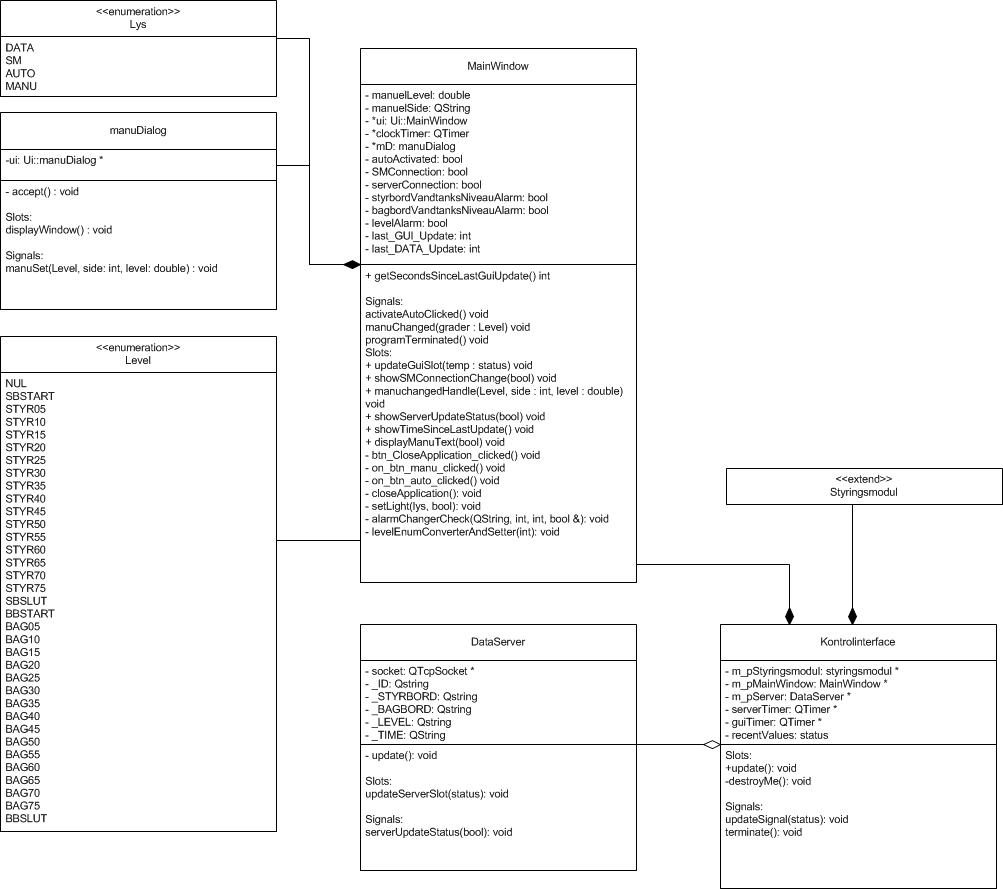
\includegraphics[width=1\textwidth]{billeder/KI-Class}
\caption{På figuren ses klassediagrammet for KI - Kontrolinterface-delen}
\end{figure}

\begin{figure}[H]
\centering
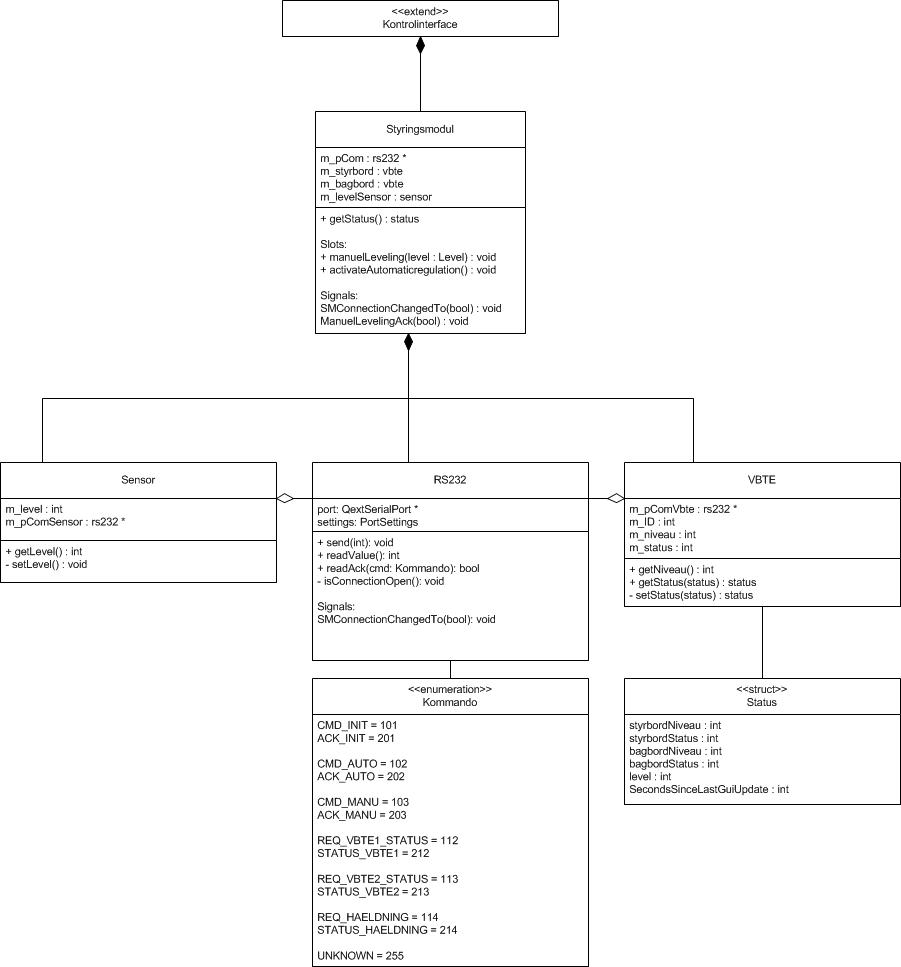
\includegraphics[width=1\textwidth]{billeder/SM-Class}
\caption{På figuren ses klassediagrammet for KI - Styringsmodul-delen}
\end{figure}

\subsection{Globale variabler}
\begin{table}[H]
\begin{tabular}{|l|p{10cm}|}
\hline
\cellcolor[gray]{0.8}\textbf{Variabel} &\cellcolor[gray]{0.8} \textbf{Beskrivelse}\\ \hline
BurstLengthVal & Denne variabel er anvendt til at håndtere antallet af perioder burstet bliver sendt med.\\ \hline
WaitBurstVar & Bliver brugt til nonblocking delay til SendBurst funktionen.\\ \hline
BurstTimerVal & Holder på Timerens værdi når et burst er sendt.\\ \hline
DistanceTimerVal & Holder værdien på timeren når et burst er modtaget. \\ \hline
CalcDistFlag & Bliver sat når et burst er modtaget så en afstand kan blive beregnet.\\ \hline
\end{tabular}
\end{table}
\subsection{Valve}
\subsubsection{Ansvar}
Denne header har til ansvar at styre ventilerne ud fra "state"-variablen modtaget fra I2C\_handle. Headeren benytter PSoC-API'et til kontrol registre..
\subsubsection{Funktionsbeskrivelser}
\textcolor{blue}{void} ChangeState( \textcolor{blue}{uint8} state ); 
\begin{table}[H]
\begin{tabular}{l p{12.5cm}}
\hline
Beskrivelse:& Funktionen anvender API'et fra I2C blokken i PSoC miljøet. Med disse tjekker den om der er fyldt nyt i bufferen og aflæse dette. Herfer kalder den funktionen I2C\_decode(); til at afkode beskeden fra SM. Herefter klargøres readbufferen til evt. at sende vandniveau tilbage. \\
Parametre:&\textcolor{blue}{uint8}* WriteBuffer\\
&\textcolor{blue}{uint8}* ReadBuffer\\
&\textcolor{blue}{uint8} BufferSize \\
Returværdi:& \textcolor{blue}{uint8} State\\
\end{tabular}
\end{table}

\subsection{Dist}
\subsubsection{Ansvar}
Denne header har til ansvar at sende burst, beregne afstanden samt at omregne afstanden til procent.
\subsubsection{Funktionsbeskrivelser}
\textcolor{blue}{void} SendBurst( \textcolor{blue}{void} );
\begin{table}[H]
\begin{tabular}{l p{12.5cm}}
\hline
Beskrivelse:&tis\\
Parametre:&hund\\
Returværdi:& henning\\
\end{tabular}
\end{table}
\subsection{Eventuelle Sekvensdiagrammer og state machines}
hab hab